% Created by tikzDevice version 0.12 on 2019-06-30 11:44:46
% !TEX encoding = UTF-8 Unicode
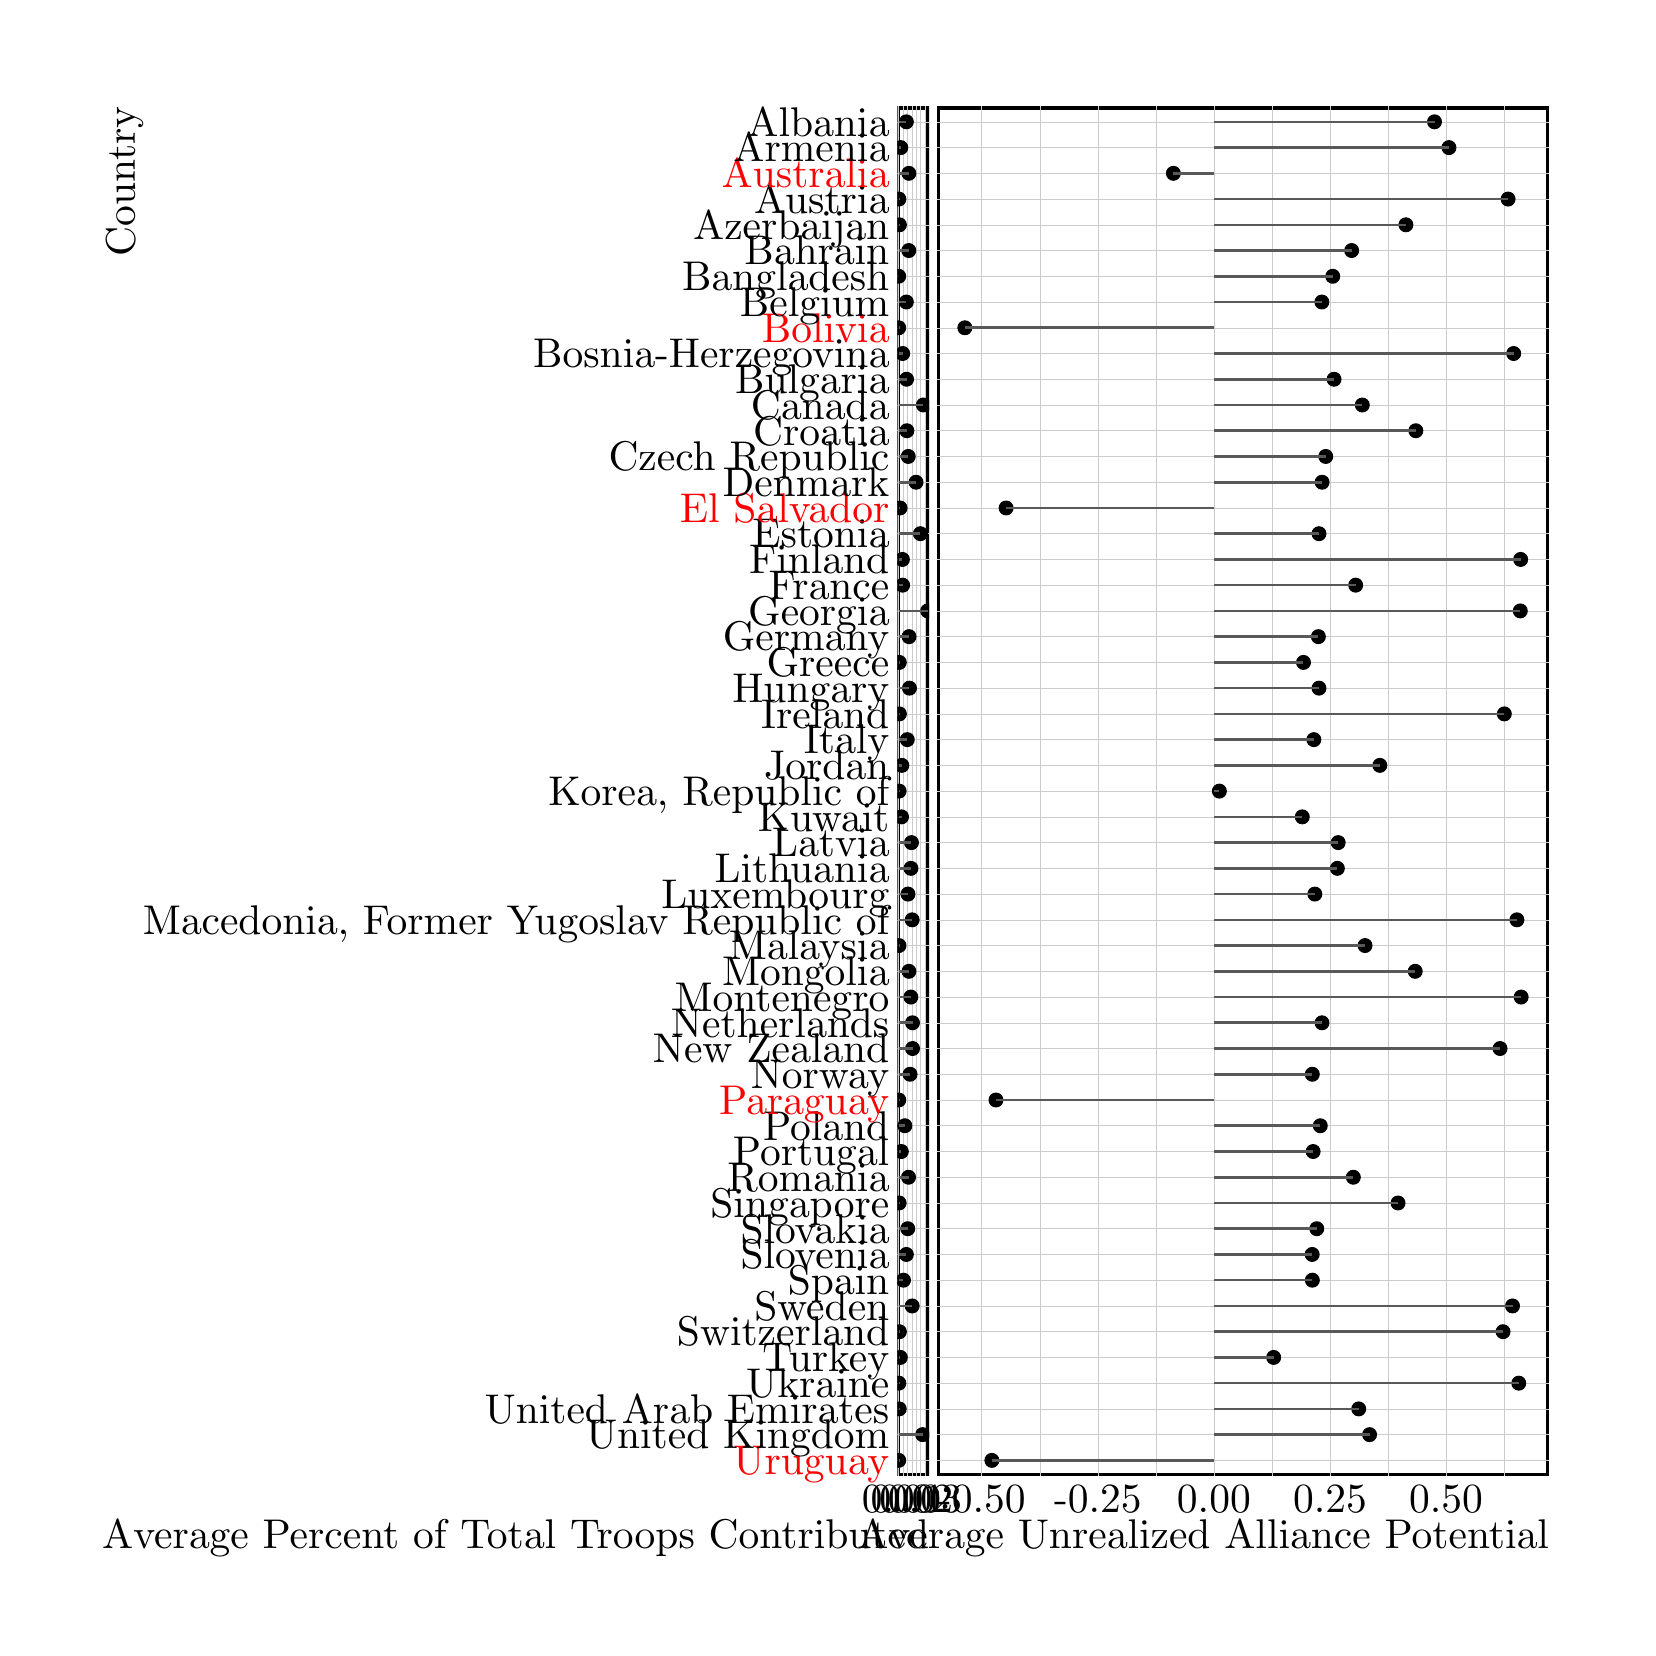
\begin{tikzpicture}[x=1pt,y=1pt]
\definecolor{fillColor}{RGB}{255,255,255}
\path[use as bounding box,fill=fillColor,fill opacity=0.00] (0,0) rectangle (578.16,578.16);
\begin{scope}
\path[clip] (314.22, 54.86) rectangle (325.72,549.71);
\definecolor{drawColor}{RGB}{0,0,0}
\definecolor{fillColor}{RGB}{255,255,255}

\path[draw=drawColor,line width= 2.3pt,line join=round,line cap=round,fill=fillColor] (314.22, 54.86) rectangle (325.72,549.71);
\definecolor{drawColor}{gray}{0.80}

\path[draw=drawColor,line width= 0.2pt,line join=round] (316.32, 54.86) --
	(316.32,549.71);

\path[draw=drawColor,line width= 0.2pt,line join=round] (319.47, 54.86) --
	(319.47,549.71);

\path[draw=drawColor,line width= 0.2pt,line join=round] (322.63, 54.86) --
	(322.63,549.71);

\path[draw=drawColor,line width= 0.2pt,line join=round] (314.22, 60.45) --
	(325.72, 60.45);

\path[draw=drawColor,line width= 0.2pt,line join=round] (314.22, 69.75) --
	(325.72, 69.75);

\path[draw=drawColor,line width= 0.2pt,line join=round] (314.22, 79.05) --
	(325.72, 79.05);

\path[draw=drawColor,line width= 0.2pt,line join=round] (314.22, 88.35) --
	(325.72, 88.35);

\path[draw=drawColor,line width= 0.2pt,line join=round] (314.22, 97.65) --
	(325.72, 97.65);

\path[draw=drawColor,line width= 0.2pt,line join=round] (314.22,106.95) --
	(325.72,106.95);

\path[draw=drawColor,line width= 0.2pt,line join=round] (314.22,116.25) --
	(325.72,116.25);

\path[draw=drawColor,line width= 0.2pt,line join=round] (314.22,125.56) --
	(325.72,125.56);

\path[draw=drawColor,line width= 0.2pt,line join=round] (314.22,134.86) --
	(325.72,134.86);

\path[draw=drawColor,line width= 0.2pt,line join=round] (314.22,144.16) --
	(325.72,144.16);

\path[draw=drawColor,line width= 0.2pt,line join=round] (314.22,153.46) --
	(325.72,153.46);

\path[draw=drawColor,line width= 0.2pt,line join=round] (314.22,162.76) --
	(325.72,162.76);

\path[draw=drawColor,line width= 0.2pt,line join=round] (314.22,172.06) --
	(325.72,172.06);

\path[draw=drawColor,line width= 0.2pt,line join=round] (314.22,181.37) --
	(325.72,181.37);

\path[draw=drawColor,line width= 0.2pt,line join=round] (314.22,190.67) --
	(325.72,190.67);

\path[draw=drawColor,line width= 0.2pt,line join=round] (314.22,199.97) --
	(325.72,199.97);

\path[draw=drawColor,line width= 0.2pt,line join=round] (314.22,209.27) --
	(325.72,209.27);

\path[draw=drawColor,line width= 0.2pt,line join=round] (314.22,218.57) --
	(325.72,218.57);

\path[draw=drawColor,line width= 0.2pt,line join=round] (314.22,227.87) --
	(325.72,227.87);

\path[draw=drawColor,line width= 0.2pt,line join=round] (314.22,237.17) --
	(325.72,237.17);

\path[draw=drawColor,line width= 0.2pt,line join=round] (314.22,246.48) --
	(325.72,246.48);

\path[draw=drawColor,line width= 0.2pt,line join=round] (314.22,255.78) --
	(325.72,255.78);

\path[draw=drawColor,line width= 0.2pt,line join=round] (314.22,265.08) --
	(325.72,265.08);

\path[draw=drawColor,line width= 0.2pt,line join=round] (314.22,274.38) --
	(325.72,274.38);

\path[draw=drawColor,line width= 0.2pt,line join=round] (314.22,283.68) --
	(325.72,283.68);

\path[draw=drawColor,line width= 0.2pt,line join=round] (314.22,292.98) --
	(325.72,292.98);

\path[draw=drawColor,line width= 0.2pt,line join=round] (314.22,302.29) --
	(325.72,302.29);

\path[draw=drawColor,line width= 0.2pt,line join=round] (314.22,311.59) --
	(325.72,311.59);

\path[draw=drawColor,line width= 0.2pt,line join=round] (314.22,320.89) --
	(325.72,320.89);

\path[draw=drawColor,line width= 0.2pt,line join=round] (314.22,330.19) --
	(325.72,330.19);

\path[draw=drawColor,line width= 0.2pt,line join=round] (314.22,339.49) --
	(325.72,339.49);

\path[draw=drawColor,line width= 0.2pt,line join=round] (314.22,348.79) --
	(325.72,348.79);

\path[draw=drawColor,line width= 0.2pt,line join=round] (314.22,358.10) --
	(325.72,358.10);

\path[draw=drawColor,line width= 0.2pt,line join=round] (314.22,367.40) --
	(325.72,367.40);

\path[draw=drawColor,line width= 0.2pt,line join=round] (314.22,376.70) --
	(325.72,376.70);

\path[draw=drawColor,line width= 0.2pt,line join=round] (314.22,386.00) --
	(325.72,386.00);

\path[draw=drawColor,line width= 0.2pt,line join=round] (314.22,395.30) --
	(325.72,395.30);

\path[draw=drawColor,line width= 0.2pt,line join=round] (314.22,404.60) --
	(325.72,404.60);

\path[draw=drawColor,line width= 0.2pt,line join=round] (314.22,413.90) --
	(325.72,413.90);

\path[draw=drawColor,line width= 0.2pt,line join=round] (314.22,423.21) --
	(325.72,423.21);

\path[draw=drawColor,line width= 0.2pt,line join=round] (314.22,432.51) --
	(325.72,432.51);

\path[draw=drawColor,line width= 0.2pt,line join=round] (314.22,441.81) --
	(325.72,441.81);

\path[draw=drawColor,line width= 0.2pt,line join=round] (314.22,451.11) --
	(325.72,451.11);

\path[draw=drawColor,line width= 0.2pt,line join=round] (314.22,460.41) --
	(325.72,460.41);

\path[draw=drawColor,line width= 0.2pt,line join=round] (314.22,469.71) --
	(325.72,469.71);

\path[draw=drawColor,line width= 0.2pt,line join=round] (314.22,479.02) --
	(325.72,479.02);

\path[draw=drawColor,line width= 0.2pt,line join=round] (314.22,488.32) --
	(325.72,488.32);

\path[draw=drawColor,line width= 0.2pt,line join=round] (314.22,497.62) --
	(325.72,497.62);

\path[draw=drawColor,line width= 0.2pt,line join=round] (314.22,506.92) --
	(325.72,506.92);

\path[draw=drawColor,line width= 0.2pt,line join=round] (314.22,516.22) --
	(325.72,516.22);

\path[draw=drawColor,line width= 0.2pt,line join=round] (314.22,525.52) --
	(325.72,525.52);

\path[draw=drawColor,line width= 0.2pt,line join=round] (314.22,534.82) --
	(325.72,534.82);

\path[draw=drawColor,line width= 0.2pt,line join=round] (314.22,544.13) --
	(325.72,544.13);

\path[draw=drawColor,line width= 0.2pt,line join=round] (314.74, 54.86) --
	(314.74,549.71);

\path[draw=drawColor,line width= 0.2pt,line join=round] (317.89, 54.86) --
	(317.89,549.71);

\path[draw=drawColor,line width= 0.2pt,line join=round] (321.05, 54.86) --
	(321.05,549.71);

\path[draw=drawColor,line width= 0.2pt,line join=round] (324.20, 54.86) --
	(324.20,549.71);
\definecolor{drawColor}{RGB}{0,0,0}
\definecolor{fillColor}{RGB}{0,0,0}

\path[draw=drawColor,line width= 0.4pt,line join=round,line cap=round,fill=fillColor] (317.51,544.13) circle (  2.50);

\path[draw=drawColor,line width= 0.4pt,line join=round,line cap=round,fill=fillColor] (315.50,534.82) circle (  2.50);

\path[draw=drawColor,line width= 0.4pt,line join=round,line cap=round,fill=fillColor] (318.42,525.52) circle (  2.50);

\path[draw=drawColor,line width= 0.4pt,line join=round,line cap=round,fill=fillColor] (314.81,516.22) circle (  2.50);

\path[draw=drawColor,line width= 0.4pt,line join=round,line cap=round,fill=fillColor] (315.00,506.92) circle (  2.50);

\path[draw=drawColor,line width= 0.4pt,line join=round,line cap=round,fill=fillColor] (318.39,497.62) circle (  2.50);

\path[draw=drawColor,line width= 0.4pt,line join=round,line cap=round,fill=fillColor] (314.74,488.32) circle (  2.50);

\path[draw=drawColor,line width= 0.4pt,line join=round,line cap=round,fill=fillColor] (317.51,479.02) circle (  2.50);

\path[draw=drawColor,line width= 0.4pt,line join=round,line cap=round,fill=fillColor] (314.75,469.71) circle (  2.50);

\path[draw=drawColor,line width= 0.4pt,line join=round,line cap=round,fill=fillColor] (316.19,460.41) circle (  2.50);

\path[draw=drawColor,line width= 0.4pt,line join=round,line cap=round,fill=fillColor] (317.58,451.11) circle (  2.50);

\path[draw=drawColor,line width= 0.4pt,line join=round,line cap=round,fill=fillColor] (323.65,441.81) circle (  2.50);

\path[draw=drawColor,line width= 0.4pt,line join=round,line cap=round,fill=fillColor] (317.69,432.51) circle (  2.50);

\path[draw=drawColor,line width= 0.4pt,line join=round,line cap=round,fill=fillColor] (318.19,423.21) circle (  2.50);

\path[draw=drawColor,line width= 0.4pt,line join=round,line cap=round,fill=fillColor] (321.01,413.90) circle (  2.50);

\path[draw=drawColor,line width= 0.4pt,line join=round,line cap=round,fill=fillColor] (315.24,404.60) circle (  2.50);

\path[draw=drawColor,line width= 0.4pt,line join=round,line cap=round,fill=fillColor] (322.57,395.30) circle (  2.50);

\path[draw=drawColor,line width= 0.4pt,line join=round,line cap=round,fill=fillColor] (316.08,386.00) circle (  2.50);

\path[draw=drawColor,line width= 0.4pt,line join=round,line cap=round,fill=fillColor] (316.16,376.70) circle (  2.50);

\path[draw=drawColor,line width= 0.4pt,line join=round,line cap=round,fill=fillColor] (325.20,367.40) circle (  2.50);

\path[draw=drawColor,line width= 0.4pt,line join=round,line cap=round,fill=fillColor] (318.48,358.10) circle (  2.50);

\path[draw=drawColor,line width= 0.4pt,line join=round,line cap=round,fill=fillColor] (314.96,348.79) circle (  2.50);

\path[draw=drawColor,line width= 0.4pt,line join=round,line cap=round,fill=fillColor] (318.63,339.49) circle (  2.50);

\path[draw=drawColor,line width= 0.4pt,line join=round,line cap=round,fill=fillColor] (314.99,330.19) circle (  2.50);

\path[draw=drawColor,line width= 0.4pt,line join=round,line cap=round,fill=fillColor] (317.84,320.89) circle (  2.50);

\path[draw=drawColor,line width= 0.4pt,line join=round,line cap=round,fill=fillColor] (315.88,311.59) circle (  2.50);

\path[draw=drawColor,line width= 0.4pt,line join=round,line cap=round,fill=fillColor] (314.89,302.29) circle (  2.50);

\path[draw=drawColor,line width= 0.4pt,line join=round,line cap=round,fill=fillColor] (315.76,292.98) circle (  2.50);

\path[draw=drawColor,line width= 0.4pt,line join=round,line cap=round,fill=fillColor] (319.36,283.68) circle (  2.50);

\path[draw=drawColor,line width= 0.4pt,line join=round,line cap=round,fill=fillColor] (319.17,274.38) circle (  2.50);

\path[draw=drawColor,line width= 0.4pt,line join=round,line cap=round,fill=fillColor] (318.10,265.08) circle (  2.50);

\path[draw=drawColor,line width= 0.4pt,line join=round,line cap=round,fill=fillColor] (319.61,255.78) circle (  2.50);

\path[draw=drawColor,line width= 0.4pt,line join=round,line cap=round,fill=fillColor] (314.84,246.48) circle (  2.50);

\path[draw=drawColor,line width= 0.4pt,line join=round,line cap=round,fill=fillColor] (318.44,237.17) circle (  2.50);

\path[draw=drawColor,line width= 0.4pt,line join=round,line cap=round,fill=fillColor] (319.13,227.87) circle (  2.50);

\path[draw=drawColor,line width= 0.4pt,line join=round,line cap=round,fill=fillColor] (319.73,218.57) circle (  2.50);

\path[draw=drawColor,line width= 0.4pt,line join=round,line cap=round,fill=fillColor] (319.75,209.27) circle (  2.50);

\path[draw=drawColor,line width= 0.4pt,line join=round,line cap=round,fill=fillColor] (318.85,199.97) circle (  2.50);

\path[draw=drawColor,line width= 0.4pt,line join=round,line cap=round,fill=fillColor] (314.77,190.67) circle (  2.50);

\path[draw=drawColor,line width= 0.4pt,line join=round,line cap=round,fill=fillColor] (316.96,181.37) circle (  2.50);

\path[draw=drawColor,line width= 0.4pt,line join=round,line cap=round,fill=fillColor] (315.69,172.06) circle (  2.50);

\path[draw=drawColor,line width= 0.4pt,line join=round,line cap=round,fill=fillColor] (318.29,162.76) circle (  2.50);

\path[draw=drawColor,line width= 0.4pt,line join=round,line cap=round,fill=fillColor] (314.90,153.46) circle (  2.50);

\path[draw=drawColor,line width= 0.4pt,line join=round,line cap=round,fill=fillColor] (318.01,144.16) circle (  2.50);

\path[draw=drawColor,line width= 0.4pt,line join=round,line cap=round,fill=fillColor] (317.51,134.86) circle (  2.50);

\path[draw=drawColor,line width= 0.4pt,line join=round,line cap=round,fill=fillColor] (316.47,125.56) circle (  2.50);

\path[draw=drawColor,line width= 0.4pt,line join=round,line cap=round,fill=fillColor] (319.61,116.25) circle (  2.50);

\path[draw=drawColor,line width= 0.4pt,line join=round,line cap=round,fill=fillColor] (314.99,106.95) circle (  2.50);

\path[draw=drawColor,line width= 0.4pt,line join=round,line cap=round,fill=fillColor] (315.34, 97.65) circle (  2.50);

\path[draw=drawColor,line width= 0.4pt,line join=round,line cap=round,fill=fillColor] (314.79, 88.35) circle (  2.50);

\path[draw=drawColor,line width= 0.4pt,line join=round,line cap=round,fill=fillColor] (314.94, 79.05) circle (  2.50);

\path[draw=drawColor,line width= 0.4pt,line join=round,line cap=round,fill=fillColor] (323.38, 69.75) circle (  2.50);

\path[draw=drawColor,line width= 0.4pt,line join=round,line cap=round,fill=fillColor] (314.75, 60.45) circle (  2.50);
\definecolor{fillColor}{gray}{0.35}

\path[fill=fillColor] (314.74, 59.98) rectangle (314.75, 60.91);

\path[fill=fillColor] (314.74, 69.28) rectangle (323.38, 70.21);

\path[fill=fillColor] (314.74, 78.58) rectangle (314.94, 79.51);

\path[fill=fillColor] (314.74, 87.88) rectangle (314.79, 88.82);

\path[fill=fillColor] (314.74, 97.19) rectangle (315.34, 98.12);

\path[fill=fillColor] (314.74,106.49) rectangle (314.99,107.42);

\path[fill=fillColor] (314.74,115.79) rectangle (319.61,116.72);

\path[fill=fillColor] (314.74,125.09) rectangle (316.47,126.02);

\path[fill=fillColor] (314.74,134.39) rectangle (317.51,135.32);

\path[fill=fillColor] (314.74,143.69) rectangle (318.01,144.62);

\path[fill=fillColor] (314.74,153.00) rectangle (314.90,153.93);

\path[fill=fillColor] (314.74,162.30) rectangle (318.29,163.23);

\path[fill=fillColor] (314.74,171.60) rectangle (315.69,172.53);

\path[fill=fillColor] (314.74,180.90) rectangle (316.96,181.83);

\path[fill=fillColor] (314.74,190.20) rectangle (314.77,191.13);

\path[fill=fillColor] (314.74,199.50) rectangle (318.85,200.43);

\path[fill=fillColor] (314.74,208.81) rectangle (319.75,209.74);

\path[fill=fillColor] (314.74,218.11) rectangle (319.73,219.04);

\path[fill=fillColor] (314.74,227.41) rectangle (319.13,228.34);

\path[fill=fillColor] (314.74,236.71) rectangle (318.44,237.64);

\path[fill=fillColor] (314.74,246.01) rectangle (314.84,246.94);

\path[fill=fillColor] (314.74,255.31) rectangle (319.61,256.24);

\path[fill=fillColor] (314.74,264.61) rectangle (318.10,265.54);

\path[fill=fillColor] (314.74,273.92) rectangle (319.17,274.85);

\path[fill=fillColor] (314.74,283.22) rectangle (319.36,284.15);

\path[fill=fillColor] (314.74,292.52) rectangle (315.76,293.45);

\path[fill=fillColor] (314.74,301.82) rectangle (314.89,302.75);

\path[fill=fillColor] (314.74,311.12) rectangle (315.88,312.05);

\path[fill=fillColor] (314.74,320.42) rectangle (317.84,321.35);

\path[fill=fillColor] (314.74,329.73) rectangle (314.99,330.66);

\path[fill=fillColor] (314.74,339.03) rectangle (318.63,339.96);

\path[fill=fillColor] (314.74,348.33) rectangle (314.96,349.26);

\path[fill=fillColor] (314.74,357.63) rectangle (318.48,358.56);

\path[fill=fillColor] (314.74,366.93) rectangle (325.20,367.86);

\path[fill=fillColor] (314.74,376.23) rectangle (316.16,377.16);

\path[fill=fillColor] (314.74,385.53) rectangle (316.08,386.46);

\path[fill=fillColor] (314.74,394.84) rectangle (322.57,395.77);

\path[fill=fillColor] (314.74,404.14) rectangle (315.24,405.07);

\path[fill=fillColor] (314.74,413.44) rectangle (321.01,414.37);

\path[fill=fillColor] (314.74,422.74) rectangle (318.19,423.67);

\path[fill=fillColor] (314.74,432.04) rectangle (317.69,432.97);

\path[fill=fillColor] (314.74,441.34) rectangle (323.65,442.27);

\path[fill=fillColor] (314.74,450.65) rectangle (317.58,451.58);

\path[fill=fillColor] (314.74,459.95) rectangle (316.19,460.88);

\path[fill=fillColor] (314.74,469.25) rectangle (314.75,470.18);

\path[fill=fillColor] (314.74,478.55) rectangle (317.51,479.48);

\path[fill=fillColor] (314.74,487.85) rectangle (314.74,488.78);

\path[fill=fillColor] (314.74,497.15) rectangle (318.39,498.08);

\path[fill=fillColor] (314.74,506.46) rectangle (315.00,507.39);

\path[fill=fillColor] (314.74,515.76) rectangle (314.81,516.69);

\path[fill=fillColor] (314.74,525.06) rectangle (318.42,525.99);

\path[fill=fillColor] (314.74,534.36) rectangle (315.50,535.29);

\path[fill=fillColor] (314.74,543.66) rectangle (317.51,544.59);
\end{scope}
\begin{scope}
\path[clip] (  0.00,  0.00) rectangle (578.16,578.16);
\definecolor{drawColor}{RGB}{255,0,0}

\node[text=drawColor,anchor=base east,inner sep=0pt, outer sep=0pt, scale=  1.50] at (311.34, 55.28) {Uruguay};
\definecolor{drawColor}{RGB}{0,0,0}

\node[text=drawColor,anchor=base east,inner sep=0pt, outer sep=0pt, scale=  1.50] at (311.34, 64.58) {United Kingdom};

\node[text=drawColor,anchor=base east,inner sep=0pt, outer sep=0pt, scale=  1.50] at (311.34, 73.88) {United Arab Emirates};

\node[text=drawColor,anchor=base east,inner sep=0pt, outer sep=0pt, scale=  1.50] at (311.34, 83.18) {Ukraine};

\node[text=drawColor,anchor=base east,inner sep=0pt, outer sep=0pt, scale=  1.50] at (311.34, 92.49) {Turkey};

\node[text=drawColor,anchor=base east,inner sep=0pt, outer sep=0pt, scale=  1.50] at (311.34,101.79) {Switzerland};

\node[text=drawColor,anchor=base east,inner sep=0pt, outer sep=0pt, scale=  1.50] at (311.34,111.09) {Sweden};

\node[text=drawColor,anchor=base east,inner sep=0pt, outer sep=0pt, scale=  1.50] at (311.34,120.39) {Spain};

\node[text=drawColor,anchor=base east,inner sep=0pt, outer sep=0pt, scale=  1.50] at (311.34,129.69) {Slovenia};

\node[text=drawColor,anchor=base east,inner sep=0pt, outer sep=0pt, scale=  1.50] at (311.34,138.99) {Slovakia};

\node[text=drawColor,anchor=base east,inner sep=0pt, outer sep=0pt, scale=  1.50] at (311.34,148.30) {Singapore};

\node[text=drawColor,anchor=base east,inner sep=0pt, outer sep=0pt, scale=  1.50] at (311.34,157.60) {Romania};

\node[text=drawColor,anchor=base east,inner sep=0pt, outer sep=0pt, scale=  1.50] at (311.34,166.90) {Portugal};

\node[text=drawColor,anchor=base east,inner sep=0pt, outer sep=0pt, scale=  1.50] at (311.34,176.20) {Poland};
\definecolor{drawColor}{RGB}{255,0,0}

\node[text=drawColor,anchor=base east,inner sep=0pt, outer sep=0pt, scale=  1.50] at (311.34,185.50) {Paraguay};
\definecolor{drawColor}{RGB}{0,0,0}

\node[text=drawColor,anchor=base east,inner sep=0pt, outer sep=0pt, scale=  1.50] at (311.34,194.80) {Norway};

\node[text=drawColor,anchor=base east,inner sep=0pt, outer sep=0pt, scale=  1.50] at (311.34,204.10) {New Zealand};

\node[text=drawColor,anchor=base east,inner sep=0pt, outer sep=0pt, scale=  1.50] at (311.34,213.41) {Netherlands};

\node[text=drawColor,anchor=base east,inner sep=0pt, outer sep=0pt, scale=  1.50] at (311.34,222.71) {Montenegro};

\node[text=drawColor,anchor=base east,inner sep=0pt, outer sep=0pt, scale=  1.50] at (311.34,232.01) {Mongolia};

\node[text=drawColor,anchor=base east,inner sep=0pt, outer sep=0pt, scale=  1.50] at (311.34,241.31) {Malaysia};

\node[text=drawColor,anchor=base east,inner sep=0pt, outer sep=0pt, scale=  1.50] at (311.34,250.61) {Macedonia, Former Yugoslav Republic of};

\node[text=drawColor,anchor=base east,inner sep=0pt, outer sep=0pt, scale=  1.50] at (311.34,259.91) {Luxembourg};

\node[text=drawColor,anchor=base east,inner sep=0pt, outer sep=0pt, scale=  1.50] at (311.34,269.22) {Lithuania};

\node[text=drawColor,anchor=base east,inner sep=0pt, outer sep=0pt, scale=  1.50] at (311.34,278.52) {Latvia};

\node[text=drawColor,anchor=base east,inner sep=0pt, outer sep=0pt, scale=  1.50] at (311.34,287.82) {Kuwait};

\node[text=drawColor,anchor=base east,inner sep=0pt, outer sep=0pt, scale=  1.50] at (311.34,297.12) {Korea, Republic of};

\node[text=drawColor,anchor=base east,inner sep=0pt, outer sep=0pt, scale=  1.50] at (311.34,306.42) {Jordan};

\node[text=drawColor,anchor=base east,inner sep=0pt, outer sep=0pt, scale=  1.50] at (311.34,315.72) {Italy};

\node[text=drawColor,anchor=base east,inner sep=0pt, outer sep=0pt, scale=  1.50] at (311.34,325.03) {Ireland};

\node[text=drawColor,anchor=base east,inner sep=0pt, outer sep=0pt, scale=  1.50] at (311.34,334.33) {Hungary};

\node[text=drawColor,anchor=base east,inner sep=0pt, outer sep=0pt, scale=  1.50] at (311.34,343.63) {Greece};

\node[text=drawColor,anchor=base east,inner sep=0pt, outer sep=0pt, scale=  1.50] at (311.34,352.93) {Germany};

\node[text=drawColor,anchor=base east,inner sep=0pt, outer sep=0pt, scale=  1.50] at (311.34,362.23) {Georgia};

\node[text=drawColor,anchor=base east,inner sep=0pt, outer sep=0pt, scale=  1.50] at (311.34,371.53) {France};

\node[text=drawColor,anchor=base east,inner sep=0pt, outer sep=0pt, scale=  1.50] at (311.34,380.83) {Finland};

\node[text=drawColor,anchor=base east,inner sep=0pt, outer sep=0pt, scale=  1.50] at (311.34,390.14) {Estonia};
\definecolor{drawColor}{RGB}{255,0,0}

\node[text=drawColor,anchor=base east,inner sep=0pt, outer sep=0pt, scale=  1.50] at (311.34,399.44) {El Salvador};
\definecolor{drawColor}{RGB}{0,0,0}

\node[text=drawColor,anchor=base east,inner sep=0pt, outer sep=0pt, scale=  1.50] at (311.34,408.74) {Denmark};

\node[text=drawColor,anchor=base east,inner sep=0pt, outer sep=0pt, scale=  1.50] at (311.34,418.04) {Czech Republic};

\node[text=drawColor,anchor=base east,inner sep=0pt, outer sep=0pt, scale=  1.50] at (311.34,427.34) {Croatia};

\node[text=drawColor,anchor=base east,inner sep=0pt, outer sep=0pt, scale=  1.50] at (311.34,436.64) {Canada};

\node[text=drawColor,anchor=base east,inner sep=0pt, outer sep=0pt, scale=  1.50] at (311.34,445.95) {Bulgaria};

\node[text=drawColor,anchor=base east,inner sep=0pt, outer sep=0pt, scale=  1.50] at (311.34,455.25) {Bosnia-Herzegovina};
\definecolor{drawColor}{RGB}{255,0,0}

\node[text=drawColor,anchor=base east,inner sep=0pt, outer sep=0pt, scale=  1.50] at (311.34,464.55) {Bolivia};
\definecolor{drawColor}{RGB}{0,0,0}

\node[text=drawColor,anchor=base east,inner sep=0pt, outer sep=0pt, scale=  1.50] at (311.34,473.85) {Belgium};

\node[text=drawColor,anchor=base east,inner sep=0pt, outer sep=0pt, scale=  1.50] at (311.34,483.15) {Bangladesh};

\node[text=drawColor,anchor=base east,inner sep=0pt, outer sep=0pt, scale=  1.50] at (311.34,492.45) {Bahrain};

\node[text=drawColor,anchor=base east,inner sep=0pt, outer sep=0pt, scale=  1.50] at (311.34,501.75) {Azerbaijan};

\node[text=drawColor,anchor=base east,inner sep=0pt, outer sep=0pt, scale=  1.50] at (311.34,511.06) {Austria};
\definecolor{drawColor}{RGB}{255,0,0}

\node[text=drawColor,anchor=base east,inner sep=0pt, outer sep=0pt, scale=  1.50] at (311.34,520.36) {Australia};
\definecolor{drawColor}{RGB}{0,0,0}

\node[text=drawColor,anchor=base east,inner sep=0pt, outer sep=0pt, scale=  1.50] at (311.34,529.66) {Armenia};

\node[text=drawColor,anchor=base east,inner sep=0pt, outer sep=0pt, scale=  1.50] at (311.34,538.96) {Albania};
\end{scope}
\begin{scope}
\path[clip] (  0.00,  0.00) rectangle (578.16,578.16);
\definecolor{drawColor}{RGB}{0,0,0}

\node[text=drawColor,anchor=base,inner sep=0pt, outer sep=0pt, scale=  1.50] at (314.74, 41.66) {0.00};

\node[text=drawColor,anchor=base,inner sep=0pt, outer sep=0pt, scale=  1.50] at (317.89, 41.66) {0.01};

\node[text=drawColor,anchor=base,inner sep=0pt, outer sep=0pt, scale=  1.50] at (321.05, 41.66) {0.02};

\node[text=drawColor,anchor=base,inner sep=0pt, outer sep=0pt, scale=  1.50] at (324.20, 41.66) {0.03};
\end{scope}
\begin{scope}
\path[clip] (  0.00,  0.00) rectangle (578.16,578.16);
\definecolor{drawColor}{RGB}{0,0,0}

\node[text=drawColor,anchor=base east,inner sep=0pt, outer sep=0pt, scale=  1.50] at (325.72, 28.45) {Average Percent of Total Troops Contributed};
\end{scope}
\begin{scope}
\path[clip] (  0.00,  0.00) rectangle (578.16,578.16);
\definecolor{drawColor}{RGB}{0,0,0}

\node[text=drawColor,rotate= 90.00,anchor=base east,inner sep=0pt, outer sep=0pt, scale=  1.50] at ( 38.78,549.71) {Country};
\end{scope}
\begin{scope}
\path[clip] (328.60, 54.86) rectangle (549.71,549.71);
\definecolor{drawColor}{RGB}{0,0,0}
\definecolor{fillColor}{RGB}{255,255,255}

\path[draw=drawColor,line width= 2.3pt,line join=round,line cap=round,fill=fillColor] (328.60, 54.86) rectangle (549.71,549.71);
\definecolor{drawColor}{gray}{0.80}

\path[draw=drawColor,line width= 0.2pt,line join=round] (365.73, 54.86) --
	(365.73,549.71);

\path[draw=drawColor,line width= 0.2pt,line join=round] (407.67, 54.86) --
	(407.67,549.71);

\path[draw=drawColor,line width= 0.2pt,line join=round] (449.60, 54.86) --
	(449.60,549.71);

\path[draw=drawColor,line width= 0.2pt,line join=round] (491.53, 54.86) --
	(491.53,549.71);

\path[draw=drawColor,line width= 0.2pt,line join=round] (533.47, 54.86) --
	(533.47,549.71);

\path[draw=drawColor,line width= 0.2pt,line join=round] (328.60, 60.45) --
	(549.71, 60.45);

\path[draw=drawColor,line width= 0.2pt,line join=round] (328.60, 69.75) --
	(549.71, 69.75);

\path[draw=drawColor,line width= 0.2pt,line join=round] (328.60, 79.05) --
	(549.71, 79.05);

\path[draw=drawColor,line width= 0.2pt,line join=round] (328.60, 88.35) --
	(549.71, 88.35);

\path[draw=drawColor,line width= 0.2pt,line join=round] (328.60, 97.65) --
	(549.71, 97.65);

\path[draw=drawColor,line width= 0.2pt,line join=round] (328.60,106.95) --
	(549.71,106.95);

\path[draw=drawColor,line width= 0.2pt,line join=round] (328.60,116.25) --
	(549.71,116.25);

\path[draw=drawColor,line width= 0.2pt,line join=round] (328.60,125.56) --
	(549.71,125.56);

\path[draw=drawColor,line width= 0.2pt,line join=round] (328.60,134.86) --
	(549.71,134.86);

\path[draw=drawColor,line width= 0.2pt,line join=round] (328.60,144.16) --
	(549.71,144.16);

\path[draw=drawColor,line width= 0.2pt,line join=round] (328.60,153.46) --
	(549.71,153.46);

\path[draw=drawColor,line width= 0.2pt,line join=round] (328.60,162.76) --
	(549.71,162.76);

\path[draw=drawColor,line width= 0.2pt,line join=round] (328.60,172.06) --
	(549.71,172.06);

\path[draw=drawColor,line width= 0.2pt,line join=round] (328.60,181.37) --
	(549.71,181.37);

\path[draw=drawColor,line width= 0.2pt,line join=round] (328.60,190.67) --
	(549.71,190.67);

\path[draw=drawColor,line width= 0.2pt,line join=round] (328.60,199.97) --
	(549.71,199.97);

\path[draw=drawColor,line width= 0.2pt,line join=round] (328.60,209.27) --
	(549.71,209.27);

\path[draw=drawColor,line width= 0.2pt,line join=round] (328.60,218.57) --
	(549.71,218.57);

\path[draw=drawColor,line width= 0.2pt,line join=round] (328.60,227.87) --
	(549.71,227.87);

\path[draw=drawColor,line width= 0.2pt,line join=round] (328.60,237.17) --
	(549.71,237.17);

\path[draw=drawColor,line width= 0.2pt,line join=round] (328.60,246.48) --
	(549.71,246.48);

\path[draw=drawColor,line width= 0.2pt,line join=round] (328.60,255.78) --
	(549.71,255.78);

\path[draw=drawColor,line width= 0.2pt,line join=round] (328.60,265.08) --
	(549.71,265.08);

\path[draw=drawColor,line width= 0.2pt,line join=round] (328.60,274.38) --
	(549.71,274.38);

\path[draw=drawColor,line width= 0.2pt,line join=round] (328.60,283.68) --
	(549.71,283.68);

\path[draw=drawColor,line width= 0.2pt,line join=round] (328.60,292.98) --
	(549.71,292.98);

\path[draw=drawColor,line width= 0.2pt,line join=round] (328.60,302.29) --
	(549.71,302.29);

\path[draw=drawColor,line width= 0.2pt,line join=round] (328.60,311.59) --
	(549.71,311.59);

\path[draw=drawColor,line width= 0.2pt,line join=round] (328.60,320.89) --
	(549.71,320.89);

\path[draw=drawColor,line width= 0.2pt,line join=round] (328.60,330.19) --
	(549.71,330.19);

\path[draw=drawColor,line width= 0.2pt,line join=round] (328.60,339.49) --
	(549.71,339.49);

\path[draw=drawColor,line width= 0.2pt,line join=round] (328.60,348.79) --
	(549.71,348.79);

\path[draw=drawColor,line width= 0.2pt,line join=round] (328.60,358.10) --
	(549.71,358.10);

\path[draw=drawColor,line width= 0.2pt,line join=round] (328.60,367.40) --
	(549.71,367.40);

\path[draw=drawColor,line width= 0.2pt,line join=round] (328.60,376.70) --
	(549.71,376.70);

\path[draw=drawColor,line width= 0.2pt,line join=round] (328.60,386.00) --
	(549.71,386.00);

\path[draw=drawColor,line width= 0.2pt,line join=round] (328.60,395.30) --
	(549.71,395.30);

\path[draw=drawColor,line width= 0.2pt,line join=round] (328.60,404.60) --
	(549.71,404.60);

\path[draw=drawColor,line width= 0.2pt,line join=round] (328.60,413.90) --
	(549.71,413.90);

\path[draw=drawColor,line width= 0.2pt,line join=round] (328.60,423.21) --
	(549.71,423.21);

\path[draw=drawColor,line width= 0.2pt,line join=round] (328.60,432.51) --
	(549.71,432.51);

\path[draw=drawColor,line width= 0.2pt,line join=round] (328.60,441.81) --
	(549.71,441.81);

\path[draw=drawColor,line width= 0.2pt,line join=round] (328.60,451.11) --
	(549.71,451.11);

\path[draw=drawColor,line width= 0.2pt,line join=round] (328.60,460.41) --
	(549.71,460.41);

\path[draw=drawColor,line width= 0.2pt,line join=round] (328.60,469.71) --
	(549.71,469.71);

\path[draw=drawColor,line width= 0.2pt,line join=round] (328.60,479.02) --
	(549.71,479.02);

\path[draw=drawColor,line width= 0.2pt,line join=round] (328.60,488.32) --
	(549.71,488.32);

\path[draw=drawColor,line width= 0.2pt,line join=round] (328.60,497.62) --
	(549.71,497.62);

\path[draw=drawColor,line width= 0.2pt,line join=round] (328.60,506.92) --
	(549.71,506.92);

\path[draw=drawColor,line width= 0.2pt,line join=round] (328.60,516.22) --
	(549.71,516.22);

\path[draw=drawColor,line width= 0.2pt,line join=round] (328.60,525.52) --
	(549.71,525.52);

\path[draw=drawColor,line width= 0.2pt,line join=round] (328.60,534.82) --
	(549.71,534.82);

\path[draw=drawColor,line width= 0.2pt,line join=round] (328.60,544.13) --
	(549.71,544.13);

\path[draw=drawColor,line width= 0.2pt,line join=round] (344.76, 54.86) --
	(344.76,549.71);

\path[draw=drawColor,line width= 0.2pt,line join=round] (386.70, 54.86) --
	(386.70,549.71);

\path[draw=drawColor,line width= 0.2pt,line join=round] (428.63, 54.86) --
	(428.63,549.71);

\path[draw=drawColor,line width= 0.2pt,line join=round] (470.57, 54.86) --
	(470.57,549.71);

\path[draw=drawColor,line width= 0.2pt,line join=round] (512.50, 54.86) --
	(512.50,549.71);
\definecolor{drawColor}{RGB}{0,0,0}
\definecolor{fillColor}{RGB}{0,0,0}

\path[draw=drawColor,line width= 0.4pt,line join=round,line cap=round,fill=fillColor] (508.35,544.13) circle (  2.50);

\path[draw=drawColor,line width= 0.4pt,line join=round,line cap=round,fill=fillColor] (513.58,534.82) circle (  2.50);

\path[draw=drawColor,line width= 0.4pt,line join=round,line cap=round,fill=fillColor] (414.00,525.52) circle (  2.50);

\path[draw=drawColor,line width= 0.4pt,line join=round,line cap=round,fill=fillColor] (534.94,516.22) circle (  2.50);

\path[draw=drawColor,line width= 0.4pt,line join=round,line cap=round,fill=fillColor] (498.01,506.92) circle (  2.50);

\path[draw=drawColor,line width= 0.4pt,line join=round,line cap=round,fill=fillColor] (478.41,497.62) circle (  2.50);

\path[draw=drawColor,line width= 0.4pt,line join=round,line cap=round,fill=fillColor] (471.58,488.32) circle (  2.50);

\path[draw=drawColor,line width= 0.4pt,line join=round,line cap=round,fill=fillColor] (467.64,479.02) circle (  2.50);

\path[draw=drawColor,line width= 0.4pt,line join=round,line cap=round,fill=fillColor] (338.65,469.71) circle (  2.50);

\path[draw=drawColor,line width= 0.4pt,line join=round,line cap=round,fill=fillColor] (536.96,460.41) circle (  2.50);

\path[draw=drawColor,line width= 0.4pt,line join=round,line cap=round,fill=fillColor] (472.05,451.11) circle (  2.50);

\path[draw=drawColor,line width= 0.4pt,line join=round,line cap=round,fill=fillColor] (482.26,441.81) circle (  2.50);

\path[draw=drawColor,line width= 0.4pt,line join=round,line cap=round,fill=fillColor] (501.60,432.51) circle (  2.50);

\path[draw=drawColor,line width= 0.4pt,line join=round,line cap=round,fill=fillColor] (469.05,423.21) circle (  2.50);

\path[draw=drawColor,line width= 0.4pt,line join=round,line cap=round,fill=fillColor] (467.73,413.90) circle (  2.50);

\path[draw=drawColor,line width= 0.4pt,line join=round,line cap=round,fill=fillColor] (353.55,404.60) circle (  2.50);

\path[draw=drawColor,line width= 0.4pt,line join=round,line cap=round,fill=fillColor] (466.61,395.30) circle (  2.50);

\path[draw=drawColor,line width= 0.4pt,line join=round,line cap=round,fill=fillColor] (539.48,386.00) circle (  2.50);

\path[draw=drawColor,line width= 0.4pt,line join=round,line cap=round,fill=fillColor] (479.87,376.70) circle (  2.50);

\path[draw=drawColor,line width= 0.4pt,line join=round,line cap=round,fill=fillColor] (539.35,367.40) circle (  2.50);

\path[draw=drawColor,line width= 0.4pt,line join=round,line cap=round,fill=fillColor] (466.39,358.10) circle (  2.50);

\path[draw=drawColor,line width= 0.4pt,line join=round,line cap=round,fill=fillColor] (461.01,348.79) circle (  2.50);

\path[draw=drawColor,line width= 0.4pt,line join=round,line cap=round,fill=fillColor] (466.61,339.49) circle (  2.50);

\path[draw=drawColor,line width= 0.4pt,line join=round,line cap=round,fill=fillColor] (533.58,330.19) circle (  2.50);

\path[draw=drawColor,line width= 0.4pt,line join=round,line cap=round,fill=fillColor] (464.75,320.89) circle (  2.50);

\path[draw=drawColor,line width= 0.4pt,line join=round,line cap=round,fill=fillColor] (488.60,311.59) circle (  2.50);

\path[draw=drawColor,line width= 0.4pt,line join=round,line cap=round,fill=fillColor] (430.62,302.29) circle (  2.50);

\path[draw=drawColor,line width= 0.4pt,line join=round,line cap=round,fill=fillColor] (460.57,292.98) circle (  2.50);

\path[draw=drawColor,line width= 0.4pt,line join=round,line cap=round,fill=fillColor] (473.55,283.68) circle (  2.50);

\path[draw=drawColor,line width= 0.4pt,line join=round,line cap=round,fill=fillColor] (473.25,274.38) circle (  2.50);

\path[draw=drawColor,line width= 0.4pt,line join=round,line cap=round,fill=fillColor] (465.11,265.08) circle (  2.50);

\path[draw=drawColor,line width= 0.4pt,line join=round,line cap=round,fill=fillColor] (538.13,255.78) circle (  2.50);

\path[draw=drawColor,line width= 0.4pt,line join=round,line cap=round,fill=fillColor] (483.25,246.48) circle (  2.50);

\path[draw=drawColor,line width= 0.4pt,line join=round,line cap=round,fill=fillColor] (501.38,237.17) circle (  2.50);

\path[draw=drawColor,line width= 0.4pt,line join=round,line cap=round,fill=fillColor] (539.66,227.87) circle (  2.50);

\path[draw=drawColor,line width= 0.4pt,line join=round,line cap=round,fill=fillColor] (467.70,218.57) circle (  2.50);

\path[draw=drawColor,line width= 0.4pt,line join=round,line cap=round,fill=fillColor] (532.04,209.27) circle (  2.50);

\path[draw=drawColor,line width= 0.4pt,line join=round,line cap=round,fill=fillColor] (464.19,199.97) circle (  2.50);

\path[draw=drawColor,line width= 0.4pt,line join=round,line cap=round,fill=fillColor] (349.89,190.67) circle (  2.50);

\path[draw=drawColor,line width= 0.4pt,line join=round,line cap=round,fill=fillColor] (467.08,181.37) circle (  2.50);

\path[draw=drawColor,line width= 0.4pt,line join=round,line cap=round,fill=fillColor] (464.49,172.06) circle (  2.50);

\path[draw=drawColor,line width= 0.4pt,line join=round,line cap=round,fill=fillColor] (479.02,162.76) circle (  2.50);

\path[draw=drawColor,line width= 0.4pt,line join=round,line cap=round,fill=fillColor] (495.18,153.46) circle (  2.50);

\path[draw=drawColor,line width= 0.4pt,line join=round,line cap=round,fill=fillColor] (465.81,144.16) circle (  2.50);

\path[draw=drawColor,line width= 0.4pt,line join=round,line cap=round,fill=fillColor] (464.15,134.86) circle (  2.50);

\path[draw=drawColor,line width= 0.4pt,line join=round,line cap=round,fill=fillColor] (464.21,125.56) circle (  2.50);

\path[draw=drawColor,line width= 0.4pt,line join=round,line cap=round,fill=fillColor] (536.54,116.25) circle (  2.50);

\path[draw=drawColor,line width= 0.4pt,line join=round,line cap=round,fill=fillColor] (533.12,106.95) circle (  2.50);

\path[draw=drawColor,line width= 0.4pt,line join=round,line cap=round,fill=fillColor] (450.23, 97.65) circle (  2.50);

\path[draw=drawColor,line width= 0.4pt,line join=round,line cap=round,fill=fillColor] (538.80, 88.35) circle (  2.50);

\path[draw=drawColor,line width= 0.4pt,line join=round,line cap=round,fill=fillColor] (480.97, 79.05) circle (  2.50);

\path[draw=drawColor,line width= 0.4pt,line join=round,line cap=round,fill=fillColor] (484.89, 69.75) circle (  2.50);

\path[draw=drawColor,line width= 0.4pt,line join=round,line cap=round,fill=fillColor] (348.41, 60.45) circle (  2.50);
\definecolor{fillColor}{gray}{0.35}

\path[fill=fillColor] (348.41, 59.98) rectangle (428.63, 60.91);

\path[fill=fillColor] (349.89,190.20) rectangle (428.63,191.13);

\path[fill=fillColor] (353.55,404.14) rectangle (428.63,405.07);

\path[fill=fillColor] (338.65,469.25) rectangle (428.63,470.18);

\path[fill=fillColor] (414.00,525.06) rectangle (428.63,525.99);

\path[fill=fillColor] (428.63, 69.28) rectangle (484.89, 70.21);

\path[fill=fillColor] (428.63, 78.58) rectangle (480.97, 79.51);

\path[fill=fillColor] (428.63, 87.88) rectangle (538.80, 88.82);

\path[fill=fillColor] (428.63, 97.19) rectangle (450.23, 98.12);

\path[fill=fillColor] (428.63,106.49) rectangle (533.12,107.42);

\path[fill=fillColor] (428.63,115.79) rectangle (536.54,116.72);

\path[fill=fillColor] (428.63,125.09) rectangle (464.21,126.02);

\path[fill=fillColor] (428.63,134.39) rectangle (464.15,135.32);

\path[fill=fillColor] (428.63,143.69) rectangle (465.81,144.62);

\path[fill=fillColor] (428.63,153.00) rectangle (495.18,153.93);

\path[fill=fillColor] (428.63,162.30) rectangle (479.02,163.23);

\path[fill=fillColor] (428.63,171.60) rectangle (464.49,172.53);

\path[fill=fillColor] (428.63,180.90) rectangle (467.08,181.83);

\path[fill=fillColor] (428.63,199.50) rectangle (464.19,200.43);

\path[fill=fillColor] (428.63,208.81) rectangle (532.04,209.74);

\path[fill=fillColor] (428.63,218.11) rectangle (467.70,219.04);

\path[fill=fillColor] (428.63,227.41) rectangle (539.66,228.34);

\path[fill=fillColor] (428.63,236.71) rectangle (501.38,237.64);

\path[fill=fillColor] (428.63,246.01) rectangle (483.25,246.94);

\path[fill=fillColor] (428.63,255.31) rectangle (538.13,256.24);

\path[fill=fillColor] (428.63,264.61) rectangle (465.11,265.54);

\path[fill=fillColor] (428.63,273.92) rectangle (473.25,274.85);

\path[fill=fillColor] (428.63,283.22) rectangle (473.55,284.15);

\path[fill=fillColor] (428.63,292.52) rectangle (460.57,293.45);

\path[fill=fillColor] (428.63,301.82) rectangle (430.62,302.75);

\path[fill=fillColor] (428.63,311.12) rectangle (488.60,312.05);

\path[fill=fillColor] (428.63,320.42) rectangle (464.75,321.35);

\path[fill=fillColor] (428.63,329.73) rectangle (533.58,330.66);

\path[fill=fillColor] (428.63,339.03) rectangle (466.61,339.96);

\path[fill=fillColor] (428.63,348.33) rectangle (461.01,349.26);

\path[fill=fillColor] (428.63,357.63) rectangle (466.39,358.56);

\path[fill=fillColor] (428.63,366.93) rectangle (539.35,367.86);

\path[fill=fillColor] (428.63,376.23) rectangle (479.87,377.16);

\path[fill=fillColor] (428.63,385.53) rectangle (539.48,386.46);

\path[fill=fillColor] (428.63,394.84) rectangle (466.61,395.77);

\path[fill=fillColor] (428.63,413.44) rectangle (467.73,414.37);

\path[fill=fillColor] (428.63,422.74) rectangle (469.05,423.67);

\path[fill=fillColor] (428.63,432.04) rectangle (501.60,432.97);

\path[fill=fillColor] (428.63,441.34) rectangle (482.26,442.27);

\path[fill=fillColor] (428.63,450.65) rectangle (472.05,451.58);

\path[fill=fillColor] (428.63,459.95) rectangle (536.96,460.88);

\path[fill=fillColor] (428.63,478.55) rectangle (467.64,479.48);

\path[fill=fillColor] (428.63,487.85) rectangle (471.58,488.78);

\path[fill=fillColor] (428.63,497.15) rectangle (478.41,498.08);

\path[fill=fillColor] (428.63,506.46) rectangle (498.01,507.39);

\path[fill=fillColor] (428.63,515.76) rectangle (534.94,516.69);

\path[fill=fillColor] (428.63,534.36) rectangle (513.58,535.29);

\path[fill=fillColor] (428.63,543.66) rectangle (508.35,544.59);
\end{scope}
\begin{scope}
\path[clip] (  0.00,  0.00) rectangle (578.16,578.16);
\definecolor{drawColor}{RGB}{0,0,0}

\node[text=drawColor,anchor=base,inner sep=0pt, outer sep=0pt, scale=  1.50] at (344.76, 41.66) {-0.50};

\node[text=drawColor,anchor=base,inner sep=0pt, outer sep=0pt, scale=  1.50] at (386.70, 41.66) {-0.25};

\node[text=drawColor,anchor=base,inner sep=0pt, outer sep=0pt, scale=  1.50] at (428.63, 41.66) {0.00};

\node[text=drawColor,anchor=base,inner sep=0pt, outer sep=0pt, scale=  1.50] at (470.57, 41.66) {0.25};

\node[text=drawColor,anchor=base,inner sep=0pt, outer sep=0pt, scale=  1.50] at (512.50, 41.66) {0.50};
\end{scope}
\begin{scope}
\path[clip] (  0.00,  0.00) rectangle (578.16,578.16);
\definecolor{drawColor}{RGB}{0,0,0}

\node[text=drawColor,anchor=base east,inner sep=0pt, outer sep=0pt, scale=  1.50] at (549.71, 28.45) {Average Unrealized Alliance Potential};
\end{scope}
\end{tikzpicture}
